\documentclass{standalone}
\usepackage{tikz}
\usetikzlibrary{patterns, positioning}


\begin{document}
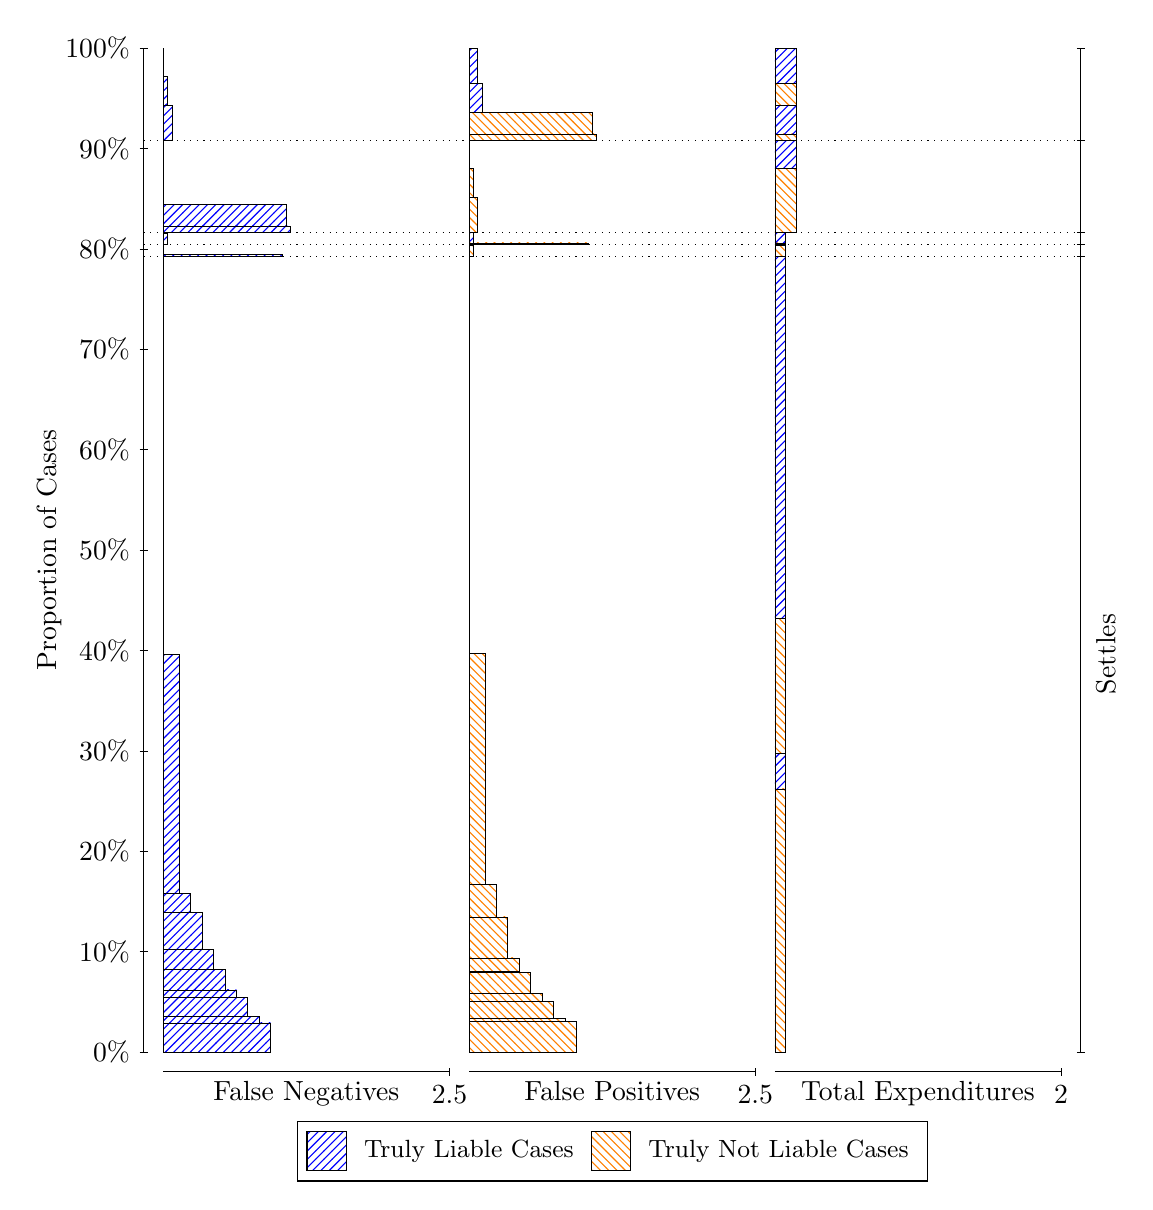
\begin{tikzpicture}
\draw[black, very thin] (1.5,1.75) -- (1.5,14.5);
\node[rotate=90, text=black, anchor=center] at (0.3, 8.125) {Proportion of Cases};
\draw[black, very thin] (1.45,1.75) -- (1.55,1.75);
\node[text=black, anchor=east] at (1.45, 1.75) {0\%};
\draw[black, very thin] (1.45,3.025) -- (1.55,3.025);
\node[text=black, anchor=east] at (1.45, 3.025) {10\%};
\draw[black, very thin] (1.45,4.3) -- (1.55,4.3);
\node[text=black, anchor=east] at (1.45, 4.3) {20\%};
\draw[black, very thin] (1.45,5.575) -- (1.55,5.575);
\node[text=black, anchor=east] at (1.45, 5.575) {30\%};
\draw[black, very thin] (1.45,6.85) -- (1.55,6.85);
\node[text=black, anchor=east] at (1.45, 6.85) {40\%};
\draw[black, very thin] (1.45,8.125) -- (1.55,8.125);
\node[text=black, anchor=east] at (1.45, 8.125) {50\%};
\draw[black, very thin] (1.45,9.4) -- (1.55,9.4);
\node[text=black, anchor=east] at (1.45, 9.4) {60\%};
\draw[black, very thin] (1.45,10.675) -- (1.55,10.675);
\node[text=black, anchor=east] at (1.45, 10.675) {70\%};
\draw[black, very thin] (1.45,11.95) -- (1.55,11.95);
\node[text=black, anchor=east] at (1.45, 11.95) {80\%};
\draw[black, very thin] (1.45,13.225) -- (1.55,13.225);
\node[text=black, anchor=east] at (1.45, 13.225) {90\%};
\draw[black, very thin] (1.45,14.5) -- (1.55,14.5);
\node[text=black, anchor=east] at (1.45, 14.5) {100\%};

\draw[black, very thin] (13.4,1.75) -- (13.4,14.5);
\draw[black, very thin] (13.35,1.75) -- (13.45,1.75);
\node[anchor=west] at (13.35, 1.75) {};
\draw[black, very thin] (13.35,11.858) -- (13.45,11.858);
\node[anchor=west] at (13.35, 11.858) {};
\draw[black, very thin] (13.35,12.008) -- (13.45,12.008);
\node[anchor=west] at (13.35, 12.008) {};
\draw[black, very thin] (13.35,12.158) -- (13.45,12.158);
\node[anchor=west] at (13.35, 12.158) {};
\draw[black, very thin] (13.35,13.325) -- (13.45,13.325);
\node[anchor=west] at (13.35, 13.325) {};
\draw[black, very thin] (13.35,14.5) -- (13.45,14.5);
\node[anchor=west] at (13.35, 14.5) {};

\draw[black, very thin, pattern color=blue, pattern=north east lines] (1.75,1.75) rectangle (3.1125,2.1182);
\draw[black, very thin, pattern color=blue, pattern=north east lines] (1.75,2.1182) rectangle (2.9672,2.2028);
\draw[black, very thin, pattern color=blue, pattern=north east lines] (1.75,2.2028) rectangle (2.8218,2.4466);
\draw[black, very thin, pattern color=blue, pattern=north east lines] (1.75,2.4466) rectangle (2.6765,2.5374);
\draw[black, very thin, pattern color=blue, pattern=north east lines] (1.75,2.5374) rectangle (2.5312,2.8025);
\draw[black, very thin, pattern color=blue, pattern=north east lines] (1.75,2.8025) rectangle (2.3858,3.0521);
\draw[black, very thin, pattern color=blue, pattern=north east lines] (1.75,3.0521) rectangle (2.2405,3.5269);
\draw[black, very thin, pattern color=blue, pattern=north east lines] (1.75,3.5269) rectangle (2.0952,3.7635);
\draw[black, very thin, pattern color=blue, pattern=north east lines] (1.75,3.7635) rectangle (1.9498,6.8002);
\draw[black, very thin, pattern color=orange, pattern=north west lines] (1.75,6.8002) rectangle (1.75,11.858);
\draw[black, very thin, pattern color=blue, pattern=north east lines] (1.75,11.858) rectangle (3.2578,11.875);
\draw[black, very thin, pattern color=orange, pattern=north west lines] (1.75,11.875) rectangle (1.75,12.008);
\draw[black, very thin, pattern color=blue, pattern=north east lines] (1.75,12.008) rectangle (1.8045,12.142);
\draw[black, very thin, pattern color=orange, pattern=north west lines] (1.75,12.142) rectangle (1.75,12.158);
\draw[black, very thin, pattern color=blue, pattern=north east lines] (1.75,12.158) rectangle (3.3668,12.242);
\draw[black, very thin, pattern color=blue, pattern=north east lines] (1.75,12.242) rectangle (3.3123,12.515);
\draw[black, very thin, pattern color=orange, pattern=north west lines] (1.75,12.515) rectangle (1.75,13.325);
\draw[black, very thin, pattern color=blue, pattern=north east lines] (1.75,13.325) rectangle (1.859,13.778);
\draw[black, very thin, pattern color=blue, pattern=north east lines] (1.75,13.778) rectangle (1.8045,14.143);
\draw[black, very thin, pattern color=orange, pattern=north west lines] (1.75,14.143) rectangle (1.75,14.5);
\draw[black, very thin, pattern color=orange, pattern=north west lines] (5.6333,1.75) rectangle (6.9958,2.1365);
\draw[black, very thin, pattern color=orange, pattern=north west lines] (5.6333,2.1365) rectangle (6.8505,2.1787);
\draw[black, very thin, pattern color=orange, pattern=north west lines] (5.6333,2.1787) rectangle (6.7052,2.3905);
\draw[black, very thin, pattern color=orange, pattern=north west lines] (5.6333,2.3905) rectangle (6.5598,2.4921);
\draw[black, very thin, pattern color=orange, pattern=north west lines] (5.6333,2.4921) rectangle (6.4145,2.7572);
\draw[black, very thin, pattern color=orange, pattern=north west lines] (5.6333,2.7572) rectangle (6.2692,2.7742);
\draw[black, very thin, pattern color=orange, pattern=north west lines] (5.6333,2.7742) rectangle (6.2692,2.9445);
\draw[black, very thin, pattern color=orange, pattern=north west lines] (5.6333,2.9445) rectangle (6.1238,3.466);
\draw[black, very thin, pattern color=orange, pattern=north west lines] (5.6333,3.466) rectangle (5.9785,3.8737);
\draw[black, very thin, pattern color=orange, pattern=north west lines] (5.6333,3.8737) rectangle (5.8332,6.808);
\draw[black, very thin, pattern color=blue, pattern=north east lines] (5.6333,6.808) rectangle (5.6333,11.858);
\draw[black, very thin, pattern color=orange, pattern=north west lines] (5.6333,11.858) rectangle (5.6878,11.992);
\draw[black, very thin, pattern color=blue, pattern=north east lines] (5.6333,11.992) rectangle (5.6333,12.008);
\draw[black, very thin, pattern color=orange, pattern=north west lines] (5.6333,12.008) rectangle (7.1412,12.025);
\draw[black, very thin, pattern color=blue, pattern=north east lines] (5.6333,12.025) rectangle (5.6878,12.158);
\draw[black, very thin, pattern color=orange, pattern=north west lines] (5.6333,12.158) rectangle (5.7423,12.607);
\draw[black, very thin, pattern color=orange, pattern=north west lines] (5.6333,12.607) rectangle (5.6878,12.969);
\draw[black, very thin, pattern color=blue, pattern=north east lines] (5.6333,12.969) rectangle (5.6333,13.325);
\draw[black, very thin, pattern color=orange, pattern=north west lines] (5.6333,13.325) rectangle (7.2502,13.409);
\draw[black, very thin, pattern color=orange, pattern=north west lines] (5.6333,13.409) rectangle (7.1957,13.682);
\draw[black, very thin, pattern color=blue, pattern=north east lines] (5.6333,13.682) rectangle (5.7968,14.048);
\draw[black, very thin, pattern color=blue, pattern=north east lines] (5.6333,14.048) rectangle (5.7423,14.5);
\draw[black, very thin, pattern color=orange, pattern=north west lines] (9.5167,1.75) rectangle (9.6529,5.0921);
\draw[black, very thin, pattern color=blue, pattern=north east lines] (9.5167,5.0921) rectangle (9.6529,5.5449);
\draw[black, very thin, pattern color=orange, pattern=north west lines] (9.5167,5.5449) rectangle (9.6529,7.2608);
\draw[black, very thin, pattern color=blue, pattern=north east lines] (9.5167,7.2608) rectangle (9.6529,11.858);
\draw[black, very thin, pattern color=orange, pattern=north west lines] (9.5167,11.858) rectangle (9.6529,11.992);
\draw[black, very thin, pattern color=blue, pattern=north east lines] (9.5167,11.992) rectangle (9.6529,12.008);
\draw[black, very thin, pattern color=orange, pattern=north west lines] (9.5167,12.008) rectangle (9.6529,12.025);
\draw[black, very thin, pattern color=blue, pattern=north east lines] (9.5167,12.025) rectangle (9.6529,12.158);
\draw[black, very thin, pattern color=orange, pattern=north west lines] (9.5167,12.158) rectangle (9.7892,12.969);
\draw[black, very thin, pattern color=blue, pattern=north east lines] (9.5167,12.969) rectangle (9.7892,13.325);
\draw[black, very thin, pattern color=orange, pattern=north west lines] (9.5167,13.325) rectangle (9.7892,13.409);
\draw[black, very thin, pattern color=blue, pattern=north east lines] (9.5167,13.409) rectangle (9.7892,13.775);
\draw[black, very thin, pattern color=orange, pattern=north west lines] (9.5167,13.775) rectangle (9.7892,14.048);
\draw[black, very thin, pattern color=blue, pattern=north east lines] (9.5167,14.048) rectangle (9.7892,14.5);
\draw[black, dotted] (1.5,11.858) -- (13.4,11.858);
\draw[black, dotted] (1.5,12.008) -- (13.4,12.008);
\draw[black, dotted] (1.5,12.158) -- (13.4,12.158);
\draw[black, dotted] (1.5,13.325) -- (13.4,13.325);
\draw[black, very thin] (1.75,1.5) -- (5.3833,1.5);
\node[text=black, anchor=north] at (3.5667, 1.5) {False Negatives};
\draw[black, very thin] (5.3833,1.45) -- (5.3833,1.55);
\node[text=black, anchor=north] at (5.3833, 1.45) {2.5};

\draw[black, very thin] (5.6333,1.5) -- (9.2667,1.5);
\node[text=black, anchor=north] at (7.45, 1.5) {False Positives};
\draw[black, very thin] (9.2667,1.45) -- (9.2667,1.55);
\node[text=black, anchor=north] at (9.2667, 1.45) {2.5};

\draw[black, very thin] (9.5167,1.5) -- (13.15,1.5);
\node[text=black, anchor=north] at (11.333, 1.5) {Total Expenditures};
\draw[black, very thin] (13.15,1.45) -- (13.15,1.55);
\node[text=black, anchor=north] at (13.15, 1.45) {2};

\node[text=black, centered, rotate=90] at (13.72, 6.8041) {Settles};





\draw (7.449999999999999,1.5) node[draw=none] (baseCoordinate) {};
\begin{scope}[align=center]
        \matrix[scale=0.5, draw=black, below=0.5cm of baseCoordinate, nodes={draw}, column sep=0.1cm]{
            \node[rectangle, draw, minimum width=0.5cm, minimum height=0.5cm, pattern color=blue, pattern=north east lines] {}; &
            \node[draw=none, font=\small, text=black] (B) {Truly Liable Cases}; &
            \node[rectangle, draw, minimum width=0.5cm, minimum height=0.5cm, pattern color=orange, pattern=north west lines] {}; &
            \node[draw=none, font=\small, text=black] (B) {Truly Not Liable Cases}; \\
            };
\end{scope}

\end{tikzpicture}
\end{document}